\chapter{Computational Mass Spectrometry Analysis}
\label{c:background}

% \textbf{Summary.} This chapter provides the necessary background knowledge to understand the basic principles of mass-spectrometry-based analysis as applied to large-scale untargeted biological studies. A particular emphasis is given to the application of mass spectrometry techniques in the field of metabolomics. For further readings on mass spectrometry as an analytical platform, the reader is directed to more comprehensive textbooks such as \cite{Hoffmann2007} and \cite{gross2006mass}. For literature surveys on the different steps that comprise an LC-MS data processing pipeline, the reader is directed to \cite{Castillo2011,Smith2014,Gika2014,Alonso2015} for metabolomics and \cite{Sandin2014, Megger2013, Smith2014} for proteomics.

This chapter provides the necessary background to understand the basic principles of mass-spectrometry-based analysis in large-scale biological studies, including the study of proteins (proteomics) and metabolites (metabolomics). Measurement technologies, such as nuclear magnetic resonance (NMR) and mass spectrometry (MS), are discussed next. A particular emphasis is given to the application of liquid chromatography mass spectrometry (LC-MS) in the field of metabolomics. The data generated from LC-MS measurements have to be processed before analysis, and we describe the steps involved in a typical data pre-processing pipeline, highlighting in particular the challenges of the alignment and identification steps.

\section{Background}

\subsection{Inside the Cell}

The three major types of macromolecules that are fundamentally essential to all life on Earth: deoxyribonucleic acid (DNA), ribonucleic acid (RNA) and proteins. The central dogma of molecular biology states that \emph{DNA is transcribed into RNA, which is translated into proteins}. Since its initial proposal, the central dogma model has been challenged and expanded to acknowledge other factors that can influence the transcription and translation processes. For instance, the reverse flow of information from RNA to DNA is possible but was not in the initial model. Nevertheless, the central dogma is broadly useful to explain how genetic information can flow in a biological system, starting from DNA to RNA to proteins. 

DNA is the basic storage unit of genetic information. In a rather simplified view, the flow of information in a biological system begins from the double-helix strands of the DNA as the starting point. A DNA strand consists of a series of linked nucleotides subunits. Each nucleotide is a molecule composed of a sugar molecule (deoxyribose), a phoshoric acid and a nitrogenous base. The base in DNA can be either adenine (A), thymine (T), guanine (G) or cytosine (C), and together they form the four well-known `alphabets' of the DNA. Bases are complementary in their pairing through hydrogen bonds, such that A pairs only with T, and G with C. It is this pairing that produces the double helix structure of the DNA. 

Regions of the DNA that code for specific proteins are called genes, however DNA is not the direct template for protein synthesis. Rather, DNA is \emph{transcribed} into RNA. The same information is encoded in RNA as its originating DNA strand, but with the crucial difference that the subunits (nucleotides) of RNA has ribose as the sugar molecule and uracil substituted in place of thymine as one of the bases. In this manner, the four alphabets of RNA are adenine (A), uracil (U), guanine (G) and cytosine (C). 

After the transcription process, a class of RNA molecules known as messenger RNA (mRNA) serves as the template for protein synthesis. Compared to the relatively inert DNA, mRNA is biochemically active and allows for genetic information to be transferred to outside the nucleus. The ribosome, a part of the translational apparatus of the cell, then reads mRNA and \emph{translates} it into proteins. A sequence of three RNA nucleotides, called a codon, encodes a particular amino acid, which is the building block of proteins. 

\subsection{Proteins and Metabolites}

Proteins serve critical roles in an organism and participate in nearly all cellular processes: performing cellular maintenance, catalysing chemical reactions and carrying other functions essential to life. Proteins also serve as the biochemical machineries involved in carrying out DNA replication and the transcription and translation processes themselves to produce more proteins. There are only 20 different types of amino acids that can be chained, through peptide bonds, to serve as the building blocks of proteins. A short chain of amino acid residues form a peptide, and in a longer chain, they fold into a fixed structure of a protein. The function of a protein is directly determined by its three-dimensional structure, and hence by the sequence of its amino acids. 

Apart from proteins, numerous other chemical reactions essential for sustaining life also happen inside a cell, including crucially, the breaking of organic compounds into energy and the production of other cellular building blocks involved in the transcription and translation processes. Together these chemical reactions comprise the \emph{metabolism} of an organism. In catabolic reactions, large organic molecules within a cell are broken into energy and smaller molecules. These serve as the input to anabolic reactions, producing the basic building blocks of a cell such as proteins and nucleic acids. Both anabolic and catabolic reactions are usually catalysed by enzymes, and together these two reactions comprise the metabolism of an organism. \emph{Metabolites} are small molecules (usually defined as less than 1000 Da) involved during or produced as the by-products of metabolism. Through the help of various enzymes, metabolites are transformed from one form to another in a series of chemical reactions as part of the metabolic pathways. Some examples of common metabolites are the various amino acids, fatty acids, vitamins, carbohydrates and many others. The overall set of metabolites that can be found within an organism is collectively called the \emph{metabolome}.

% The key processes involved in some of the most important life-sustaining transformations in the cell, such as for instance, the breaking of organic compounds into energy and the production of cellular building blocks (used in the other parts of the central dogma) are generally called metabolism. Metabolites are the set of small molecules produced as the by-product of metabolism. 

\subsection{The Layers of -omics}

\begin{figure}
\noindent \begin{centering}
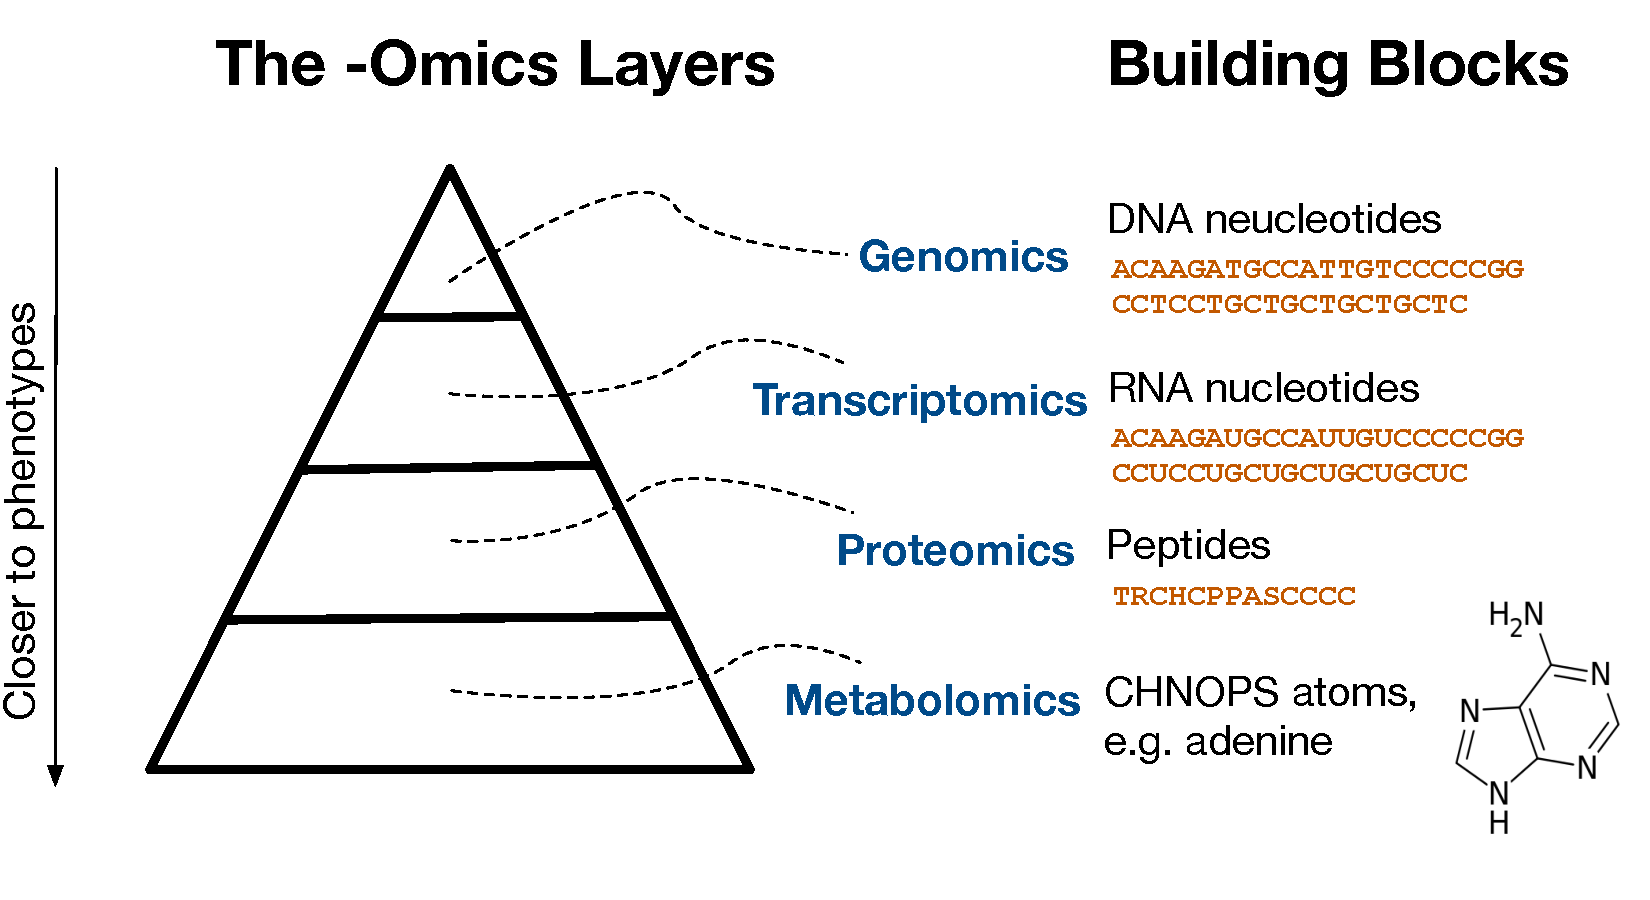
\includegraphics[width=1.0\textwidth]{02-background/figures/omics}
\par\end{centering}
\caption{\label{fig:omics-triangle}The layers of -omics and their building blocks.}
\end{figure}

As illustrated in Figure~\ref{fig:omics-triangle}, each sub-field of computational biology focuses on the entities and processes involved in a stage of the central dogma. Genomics is concerned with the large-scale study of the entire DNA in an organism (the genome) and how the genes encoded in the genome interact with each other. Transcriptomics focuses on understanding the large-scale analysis of mRNA (the transcriptome), particularly those that correspond to protein-encoding genes and measurements on their abundance in the sample. Proteins and their large-scale identifications and quantifications are studied in proteomics. Metabolomics studies the metabolome on a large scale, usually for the purpose of identifying and quantifying the differences of metabolite compositions in a particular organism or tissue under various experimental or physiological conditions. 

Moving through the successive -omics layers in Figure~\ref{fig:omics-triangle} and getting closer the physically observed properties (phenotypes) introduce greater complexity due to the increased number of ways of putting the building blocks of each -omics layer together. The building blocks of the genome are the nucleotides of the DNA, while in the transcriptome, the building blocks are the nitrogenous bases that comprise the RNA. There are only four possible bases in the genome and the transcriptome. In proteomics, the object of interest, proteins, is a chain of amino acid residues, with 20 possible amino acids to choose from. The small molecules in metabolomics have \textbf{C}arbon, \textbf{H}ydrogen, \textbf{N}itrogen, \textbf{O}xygen, \textbf{P}hospor and \textbf{S}ulphur (CHNOPS) atoms as their building blocks, which can be arranged in many chemically-plausible configurations. 

Unlike the genome that is relatively static, the proteome and metabolome of an organism are considerably more dynamic. The expression of proteins and metabolites are governed by various complex, interacting factors. In a process called post-translational modification \cite{mann2003proteomic}, proteins can be chemically modified after synthesis in a way that completely alters their structure and folding stability, e.g. through phosphorylation (the addition of a phoshate group) or methylation (the addition of a methyl group). Metabolites expression can also change in response to the cellular sytems cellular \cite{Panopoulos2012} or environmental factor \cite{Hirai2004}. As a result, the knowledge of the DNA sequence alone is not sufficient to predict the proteins and metabolites that may be expressed in an organism. The metabolome is considered closest to the phenotype \cite{Fiehn2002}, so changes to the phenotype are often most readily observed in the metabolome. Studying the metabolome therefore provides us with an instantaneous `snapshot' of chemical activities that occur in the cell, leading to an understanding of how cellular processes behave and possibly an explanation of how certain phenotypes are expressed.

\section{Measurement Technologies\label{sub:mass-spec}}

Nuclear magnetic resonance (NMR) spectroscopy and mass spectrometry (MS) are the two widely used measurement technologies for proteomics and metabolomics. NMR and MS are described in the following section, but here we provide a brief comparison of the two methods. The main advantage of NMR spectroscopy over MS is that its spectra have very high reproducibility since the same compound structure always produces peaks at the same locations in the spectra. Absolute quantification of the abundance of the compounds is possible in NMR as the signal intensity in NMR spectra is directly proportional to the concentration of protons in the nucleus of the compounds. In MS, often only the relative abundance (with respect to some reference compounds of known concentration) can be obtained. For small molecule (metabolite) analysis, while the resulting spectra from NMR provide information on the structure of the metabolites, certain regions in the spectra can also be crowded with many overlapping metabolite signals \cite{Pan2007}, potentially hindering identification. NMR also has a lower sensitivity than mass spectrometry, which limits the number of metabolites that can be detected from NMR spectra. 

The two approaches of NMR and MS are often seen as complementary rather than competitive. For more detailed comparisons of NMR vs. MS, see \cite{Pan2007}. In the following section, NMR is only briefly described since it is not the focus of this thesis, while mass spectrometry is described in greater detail.

\subsection{Nuclear Magnetic Resonance}

NMR spectroscopy operates on the principle of measuring the energy absorption of nuclei in the atom as electromagnetic radiation is applied. Atoms are the building blocks of matters, and two or more atoms connected via chemical bonds comprise a compound. An atom has a nucleus at the centre, which consists of positively charged protons and neutrons with no charge. Electrons, having negative charge, are bound to the neucleus through electromagnetic force. The overall charge of the atom is therefore determined by the number of electrons and protons that it has. An atom is called a positive ion when there are more protons than electrons, while the opposite is called a negative ion. The nucleus of an atom also possesses an angular moment, called spin. A nucleus with a positive spin develops a magnetic field, and when placed in an external magnetic field, the nucleus can either align itself with the external field (a lower energy state) or against the external field (a higher energy state). 

In NMR spectroscopy, initially most nuclei will be in their ground state of being in alignment with the external magnetic field, but when radio waves are applied, the nuclei in the lower energy state can absorb the energy and move to the higher energy state (their spin flip). When the radio waves are removed, the energised nuclei relaxes back to the lower energy state. The fluctuation of the magnetic field during relaxation is called `resonance' and can be measured in the form of a current in the magnetic coil around the sample. From NMR measurements, signals in the time-domain are obtained, and through Fourier transformation, this signal is converted from the time domain to the frequency domain. Before statistical analysis can be performed, the resulting NMR spectra are processed in a data pre-processing pipeline. This includes steps like baseline correction, noise filtering, alignment, and compound identification \cite{Alonso2015}. For identification, spectra are annotated through comparisons to databases that contain reference spectra either developed in-house or publicly available (e.g. BioMagResBank \cite{Ulrich01012008}, Madison Metabolomics Consortium Database \cite{cui2008metabolite}, and many others). Identification is one of the greatest challenges in NMR analysis \cite{Pan2007}, although in recent years, several methods such as BATMAN \cite{hao2012batman} and IQNMR \cite{song2011iqmnmr} have been introduced that aim to automate this process.

\subsection{Mass Spectrometry}

As an alternative to NMR spectroscopy, mass spectrometry operates by ionising compounds in the sample, producing charged ions that are separated by their mass-to-charge (m/z) ratio. The molecular mass of a compound is the sum of the molecular mass of its elements, measured in Daltons (Da), where one Da is $\frac{1}{12}$ of the molecular mass of the carbon element ($^{12}C$). During mass spectrometry, the compounds to be analysed (metabolites or peptide fragment) are introduced into the ionisation source of the MS, and depending on the ionisation mode used, these compound produce positively or negatively charged ions. They travel through the mass analyser and arrive at the detector at a different rate due to each ion having different mass-to-charge ratios. The detector measures the ions that arrive and produce signals in the form of a mass spectrum, showing the relative abundance of detected ions at different m/z ratios. 

Modern high-precision MS instruments have very high resolving power, with accuracy up to several parts-per-million. MS instruments can be ranked in ascending order by the resolving powers of their mass analyser: \textbf{(1)} time-of-flight MS, \textbf{(2)} orbitrap MS, and lastly \textbf{(3)} Fourier transform ion-cyclotron MS. In time-of-flight MS, ions are accelerated in an electric field. The m/z ratio of an ion is measured from how long the ion reaches the detector at a known distance. In orbitrap MS, ions are trapped in an orbital motion around an electrode. Currents are generated from the trapped ions and, through Fourier transform, converted to a mass spectrum. In ion-cyclotron MS, ions are trapped and excited in a magnetic field, inducing a charge that is transformed into mass spectrum. 

A higher resolving power corresponds to a better ability of the MS instrument to detect small differences in m/z ratios. Having a higher resolving power is generally very useful when trying to identify which metabolites are present in the sample as spectral peaks close in m/z values can be resolved, allowing for e.g. a broad peak at low resolution to be measured as multiple sharp peaks in high resolution. The difference between the observed m/z value to the exact m/z value of a compound is known as the mass accuracy of a mass spectrometry instrument, measured in parts-per-million, i.e. $\text{mass accuracy} = 1,000,000 * \frac{(\text{observed m/z} - \text{exact m/z})}{\text{exact m/z}}$. In this manner, compounds with identical nominal (integer) masses but different exact masses can be distinguished, allowing for greater confidence that a measured peak represent an actual distinct molecular species. 

In direct injection mass spectrometry, the sample is introduced into the MS at a constant flow. However the ionisation capacity of MS is limited, and in what is called the ion supression effect, compounds can compete for charges during ionisation --- resulting in some compounds not being ionised and detected in the mass spectra \cite{Smith2014}. Separating compounds as they pass through (elute) from the chromatographic column at a different \emph{retention times} (RTs) into the MS is often preferred. Additionally, from chromatographic separation, the retention time of an observed peak reflects the underlying biochemistry of the compound and can serve as an additional piece of information to deduce its identity \cite{Cao2015}. Particularly in large-scale untargeted studies, MS is often coupled to a chromatographic separation technology such as liquid chromatography (LC), forming the combined set-up of LC-MS (Figure~\ref{fig:LC-MS-setup}). 

\begin{figure}
\noindent \begin{centering}
\includegraphics[width=1.0\textwidth]{02-background/figures/LCMS}
\par\end{centering}
\caption[A typical LC-MS set-up.]{\label{fig:LC-MS-setup}A typical LC-MS set-up. High performance liquid chromatography instruments are used to separate metabolites (by their chemical properties) in the sample before they are gradually introduced into the mass spectrometer.}
\end{figure}

As illustrated in Figure~\ref{fig:LC-MS-setup}, during liquid chromatography, the solvent containing the analytes (metabolites) is introduced and pumped into the stationary phase that is part of the chromatographic column. Metabolites elute at different times due to their different interactions with the column, based on their biochemical properties (e.g. their hydrophobicity, polarity, molecular shapes etc). In the LC-MS set-up, metabolites that elute from liquid chromatography are then vaporised and ionised inside the mass spectrometer. Ionisation in an LC-MS setup is usually performed via electrospray ionisation (ESI). In ESI, the sample analyte is dissolved into a solvent and sprayed through an electrospray (a highly charged needle) creating charged droplets. In the ionisation source, the charged droplets evaporate, creating charged electric fields on their surfaces. Due to the strong electric field of the MS, ions on the surface of the droplets have enough energy to separate, generating charged molecular ions. The generated ions are separated by the mass analyser inside the MS instrument according to their m/z ratios and the detected signal abundance for a particular m/z value. As ESI requires a continuous supply of dissolved analytes, it can be directly coupled to LC. This results in the commonly-used combined liquid chromatography mass spectrometry (LC-MS) set-up. 

In the next section, we describe the data produced from LC-MS measurements and the necessary pre-processing required before the data can be used for further analysis.

\section{LC-MS Analysis in Metabolomics}

The raw data produced from an LC-MS set-up is a collection of mass spectra from each scan over a range of elution times. Each MS measurement of compounds that elute at the same or similar retention time is called a scan. A mass spectrum in each scan is the two dimensional representation of m/z values of charged ions to signal intensities (Figure~\ref{fig:LC-MS-data}C). The sum the signal intensities across all mass spectra, called the total ion chromatogram or TIC (Figure~\ref{fig:LC-MS-data}D) shows how compounds elute over time over all m/z values. The TIC plot can be crowded, so given a specific m/z range to inspect, the extracted ion chromatogram (EIC) plot shows the total signal in that m/z range vs. RT (Figure~\ref{fig:LC-MS-data}E). The m/z range for inspection in the EIC is usually selected based on the prior knowledge of what signal a compound is supposed to produce in the spectra.

\begin{figure}
\noindent \begin{centering}
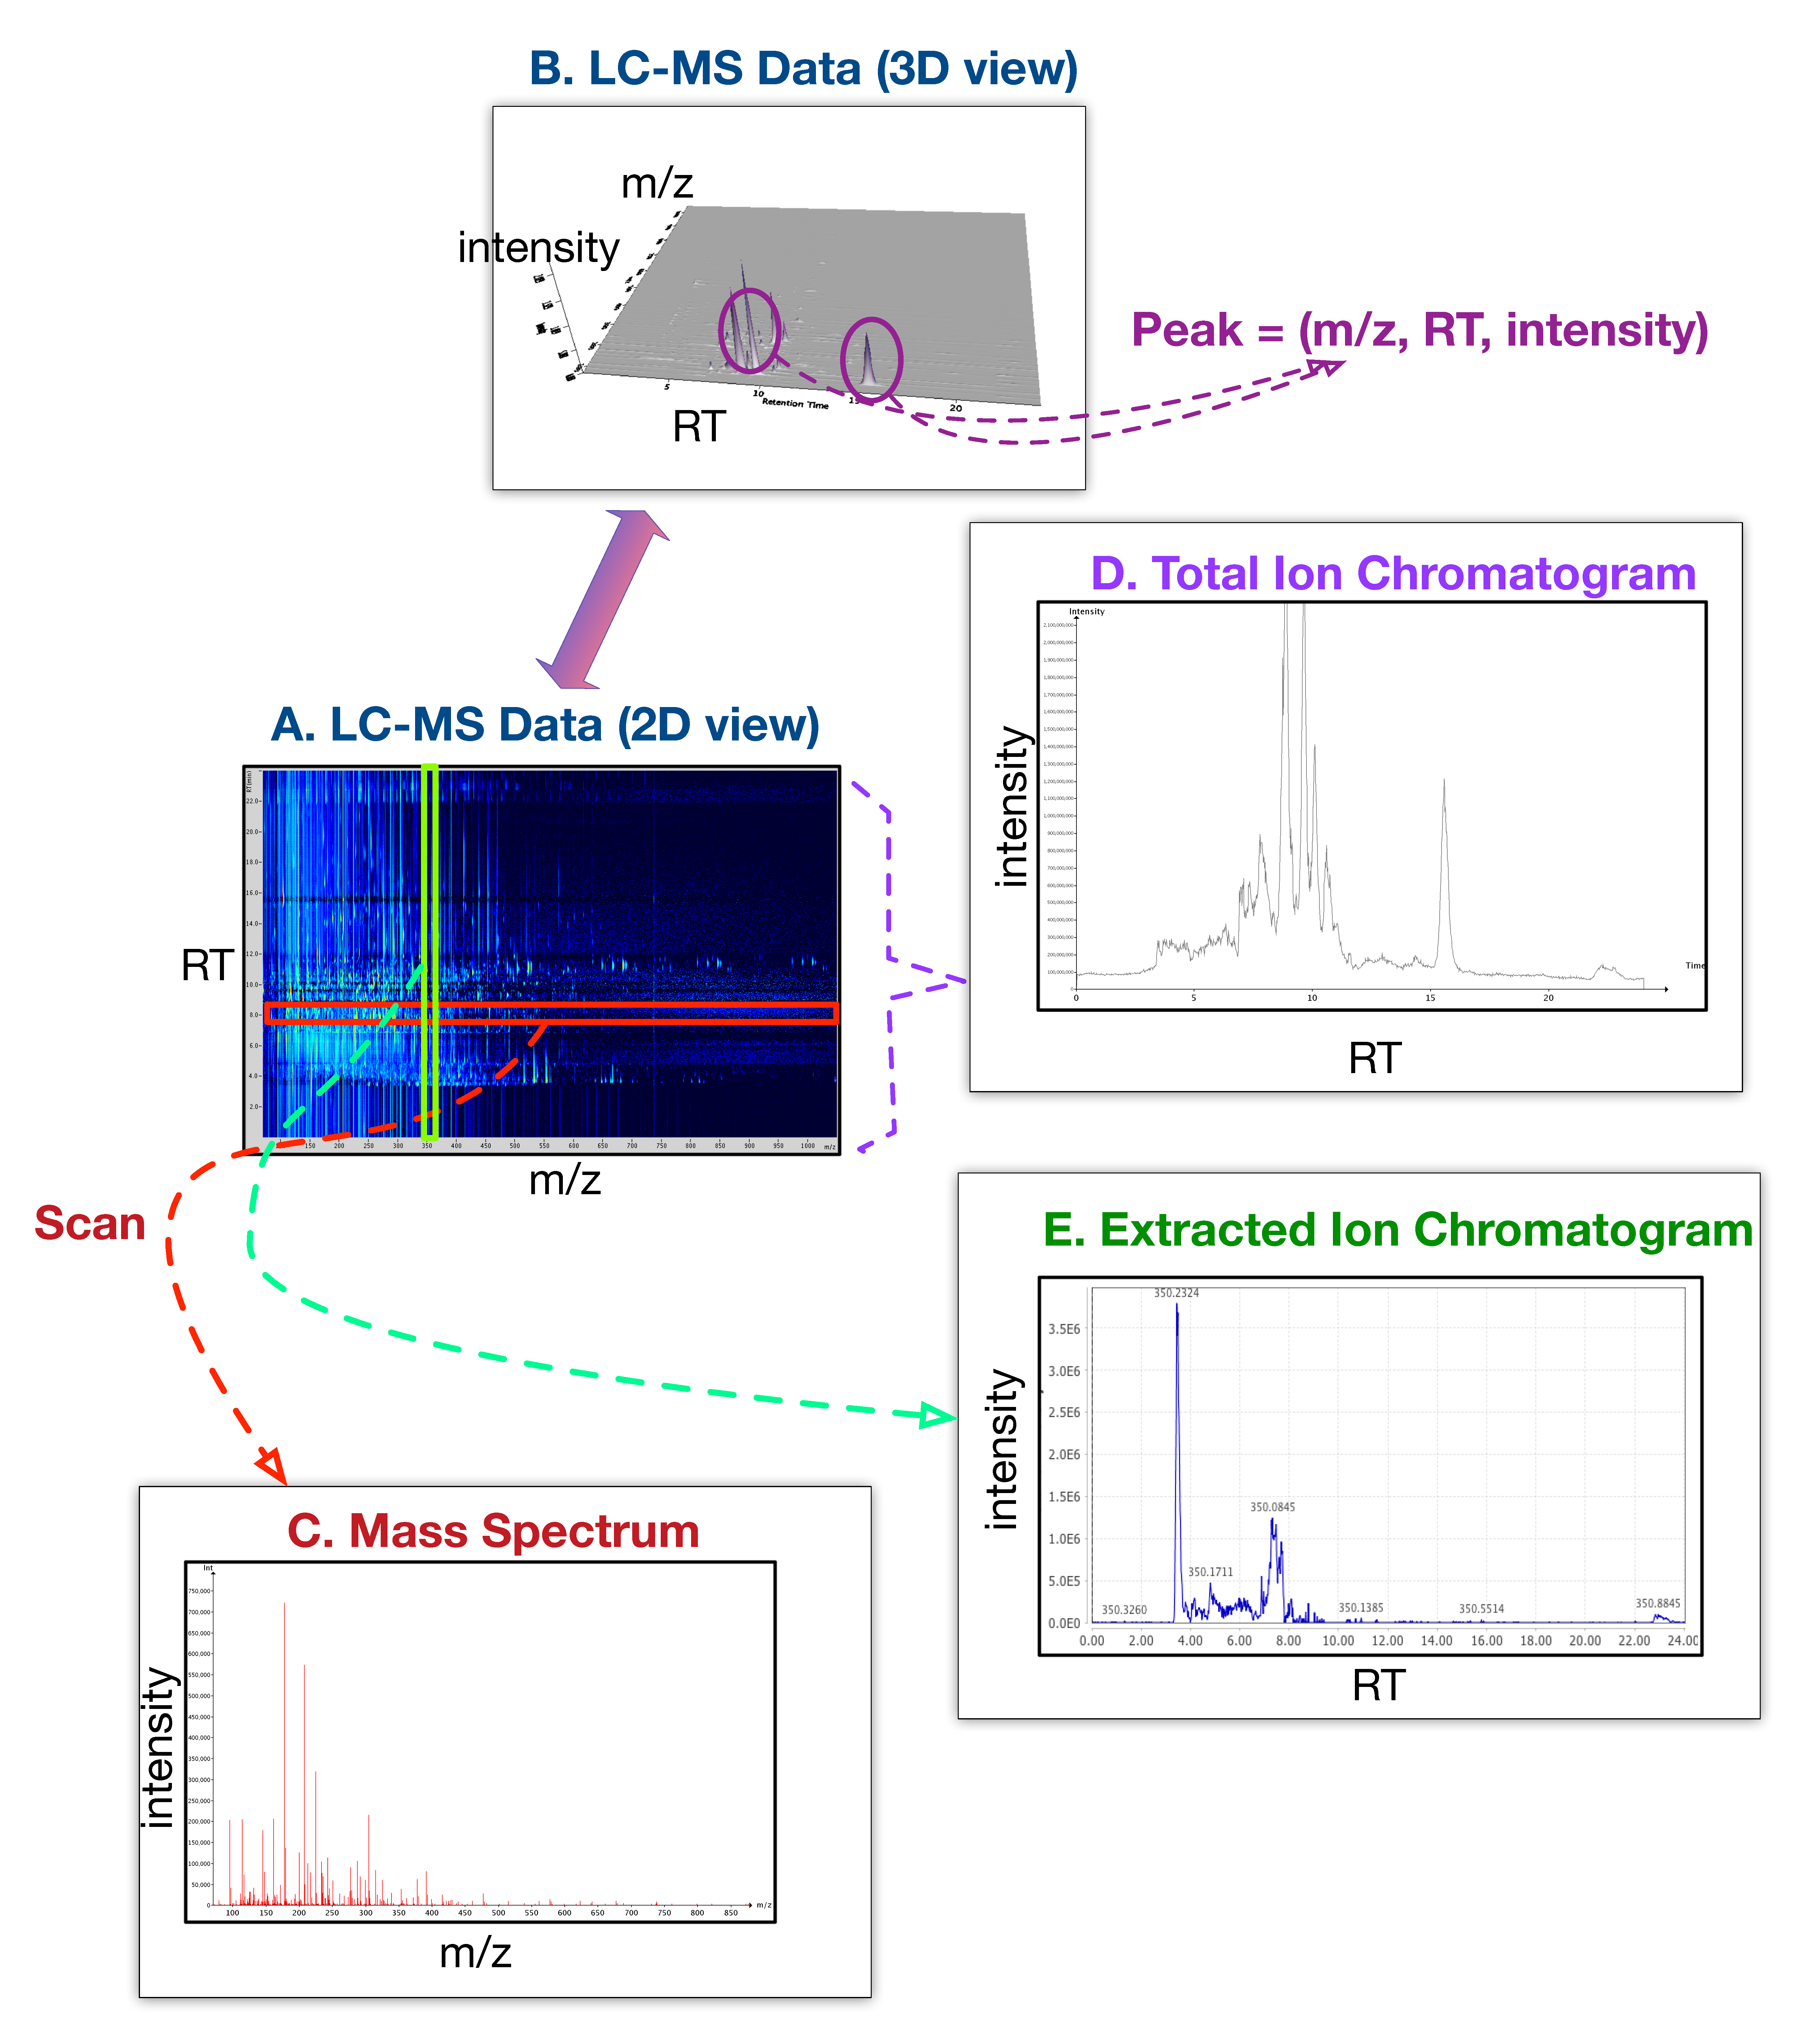
\includegraphics[width=1.0\textwidth]{02-background/figures/spectra.pdf}
\par\end{centering}
\caption[The resulting data produced from an LC-MS experiment.]{\label{fig:LC-MS-data}The resulting raw data (ion chromatograms) produced from an LC-MS experiment. We can view the data as a 2D profile seen from the top \textbf{(A)} or a 3D profile \textbf{(B)}. A peak in the data is thus characterised by its intensity value on the m/z and retention time axes. From a scan, a slice of the data on the m/z axis is the mass spectrum \textbf{(C)}. A collection of mass spectra is produced over the whole range of retention time. Summing over all scans produce the total ion chromatogram (TIC) \textbf{(D)}, while plotting the intensity values vs. RT for a particular m/z range produces the extracted ion chromatogram (EIC) \textbf{(E)}.}
\end{figure}

As shown in Figure~\ref{fig:LC-MS-data}B, the raw LC-MS data can also be viewed as a 3D image, containing peaks characterised by a set of vectors of m/z, retention time and intensity. This raw LC-MS data is noisy, so pre-processing has to take place before analysis can be performed and biological conclusion drawn. Generally, the main steps of LC-MS data pre-processing takes the form of a sequential pipeline shown in Figure~\ref{fig:pipeline}. Note that Figure~\ref{fig:pipeline} illustrates an example pipeline. In practice, many variations of this example pipeline exists. For instance, the gap filling and the peak grouping steps can be omitted, the noise filtering step can be performed before peak alignment, the pipeline may produce no visualisations. The following sections explain in detail the key steps of the LC-MS data processing pipeline in Figure~\ref{fig:pipeline}.

\begin{figure}
\noindent \centering{}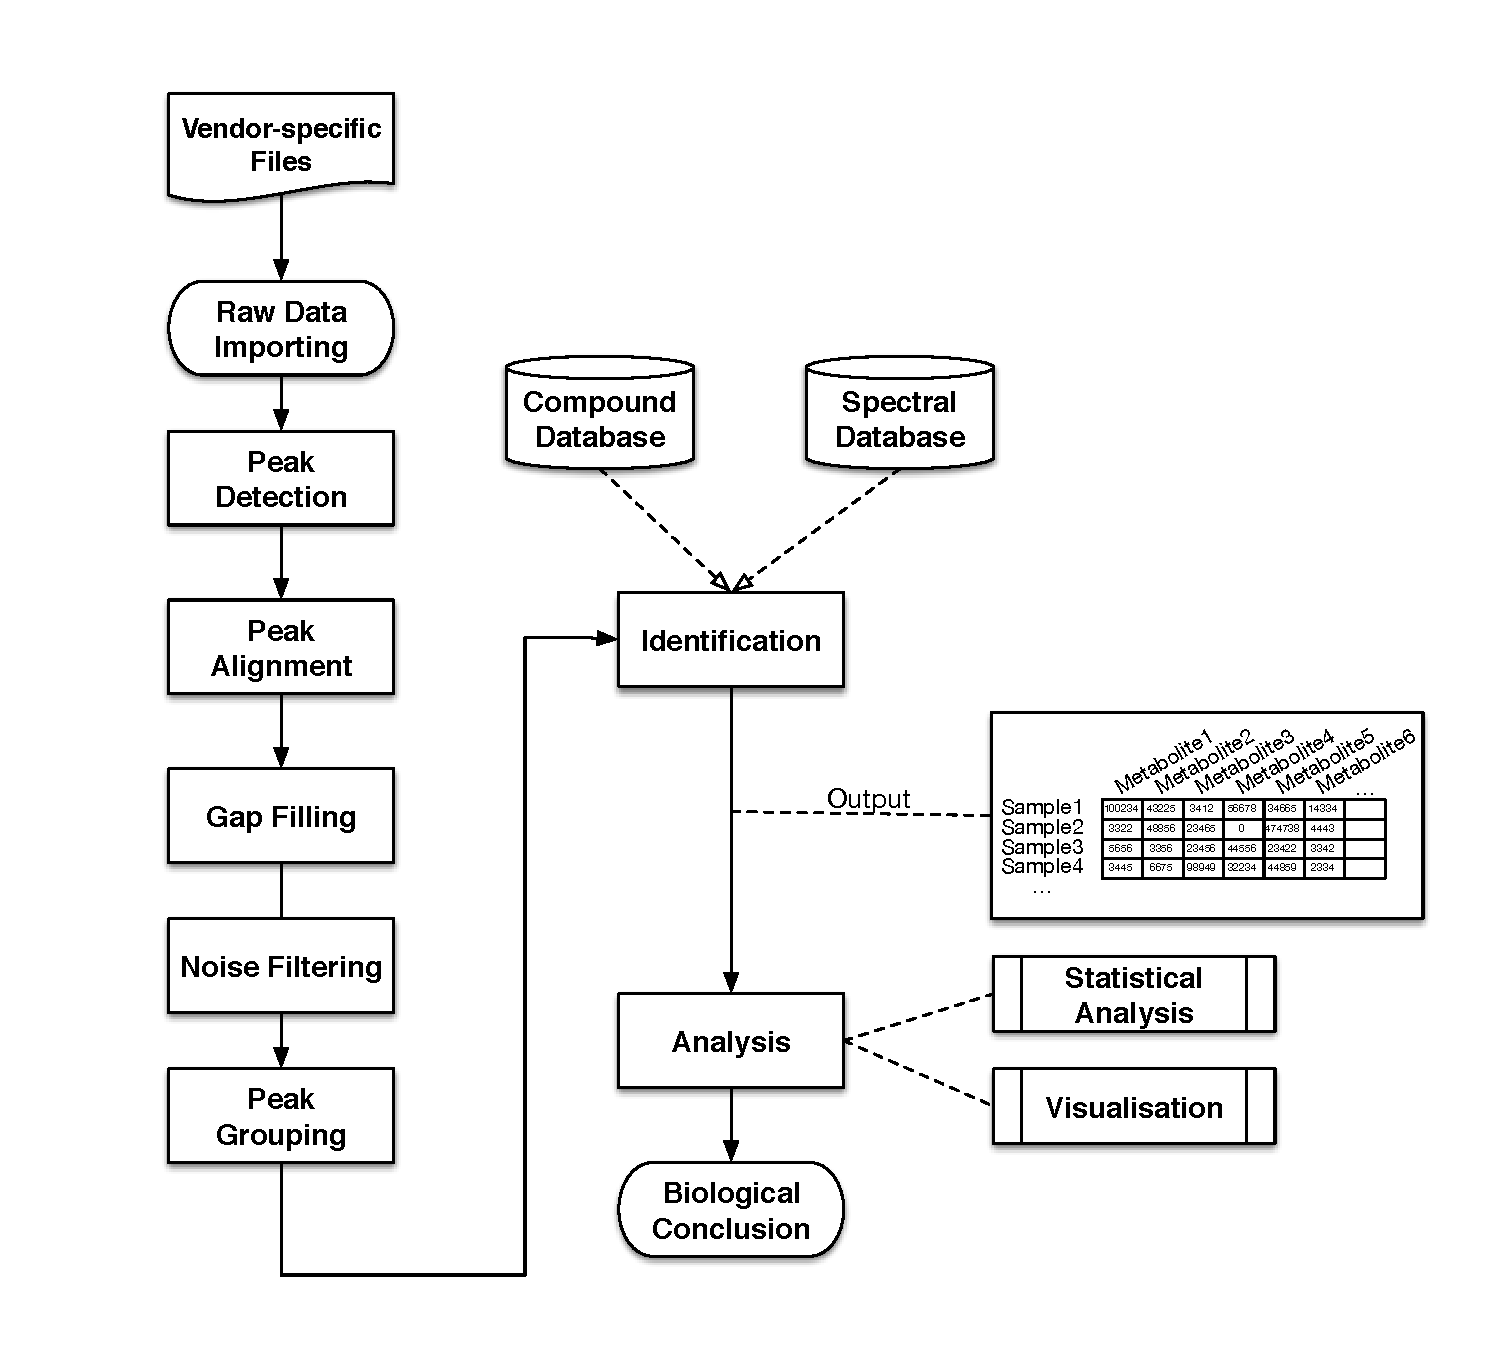
\includegraphics[width=1\textwidth]{02-background/figures/pipeline.pdf}\caption{\label{fig:pipeline}An example pre-processing pipeline of LC-MS metabolomics data.}
\end{figure}

\subsection{Raw Data Importing \& Peak Detection}

The raw data produced from measurements are generally available in vendor-proprietary format. An LC-MS data pre-processing pipeline that is based on open softwares usually starts with the importing of these proprietary files into an open XML-based format, such as mzXML \cite{Pedrioli2004} or mzML format \cite{martens2011mzml}. Peak detection is applied to the imported LC-MS data to produce peaks. Each peak feature is characterised by its m/z, RT and intensity values. The CentWave algorithm \cite{Tautenhahn2008} from XCMS is one of the more widely used peak detection method in metabolomics. It is particularly suitable for modern metabolomics data that are generated from instruments having a high mass accuracy. CentWave extracts regions of interest from the data. Chromatographic analysis of the EIC from each region of interest is performed using continuous wavelet transform and is used to detect candidate chromatographic peaks. For each candidate peak, once its chromatographic peak boundaries have been identified, the centroid m/z value of a peak feature is defined as the weighted mean of the m/z values within the boundaries. Similarly, the intensity of a peak feature is defined as the maximal intensity value in the chromatographic peak boundaries. The signal-to-noise ratio of each candidate peak is calculated and if it is lower than the thresholded defined by the user, the candidate peak is rejected. As an alternative peak detection method, the MZmine 2 \cite{Pluskal2010} software suite is also widely used. 

A survey of the many different approaches for peak detections can be found in \cite{Katajamaa2007,Castillo2011,Alonso2015}, however it is important to note that most peak detection methods are sensitive to the choice of parameters \cite{Tautenhahn2008}, with a method potentially producing different results when its parameters are varied. For instance, CentWave requires as user-defined parameters the mass deviation in parts-per-million (which is usually set based on the mass accuracy of instrument), the minimum width of the chromatographic peak and a signal-to-noise threshold. Setting a width that is too narrow or a signal-to-noise threshold that is too high can potentially lead to missing peaks. 

\subsection{Peak Alignment\label{sub:alignment-tools}}

Following peak detection, peak alignment is performed to match peaks that are the same across samples. An alignment method takes as input multiple lists of peaks --- one from each LC-MS run --- and produces as output a list of \emph{aligned peaksets}. Each aligned peakset is a set of peaks coming from different runs that are considered to be \emph{correspondent} and have to be matched. Alignment is necessary because experiments in biology usually involve the comparison of multiple samples. Samples can be produced as either biological or technical replicates. Biological replicates are obtained from the same organism studied under varying conditions and exposed to different factors (e.g. treatment or no treatment). Biological replicates are necessary to determine entities that are differentially expressed across samples. In contrast, technical replicates are obtained from the same sample analysed multiple times. Technical replicates are necessary to account for the variability and measurement errors throughout the experiment. In this manner, each replicate, whether biological or technical, is measured through the LC-MS instrument. This produces an LC-MS run for each replicate.

\subsection{Labelled Alignment}

Standards are compounds of known concentration that produce peaks at well-defined m/z and RT values. Since they are known, peaks generated from standards can be used as the `landmark' peaks to determine how retention time shift occur across samples. This simplifies the problem of alignment for these limited number of standard compounds that can be spiked into the samples before running them through LC-MS. Alternatively, stable-isotope labelling experiments exploit the fact that atoms occur as isotopes. Two isotopes of the same atom are naturally occurring elements that have the same number of protons (same atomic number) but different number of neutrons (different molecular masses). An element can have several isotope species, which occur at different abundances in nature. For instance carbon has two isotopes: $^{12}C$ with molecular mass 12.000000 at 98.890\% abundance in nature, and $^{13}C$ with molecular mass 13.003355 and 1.110\% abundance. 

When measured in mass spectrometry, isotopes in the compound produce a distinct pattern of peaks that follow the binomial distribution. This information can be used to aid peak alignment and identification. In a labelling experiment, two samples are prepared: one from cells that grow in a normal medium and another from cells that grow in isotopic reagents. The two samples are combined and measured as a single LC-MS run. A metabolite from the normal medium and its corresponding isotopic counterpart have the same chemical formula and structure and hence will appear at close retention time, however the distinctive pattern of peaks produced from the isotopic metabolite makes it possible to trace the peaks back to the metabolite that produce them \cite{chokkathukalam2014stable}. This makes alignment easier. However, labelled experiments consume expensive reagents, are more difficult to prepare and harder to compare across laboratories and to various mass spectral databases online for identification. 

\subsection{Label-free Alignment}

It is common for large-scale untargeted LC-MS experiments, where the identities of the metabolites of interest are not known in advance, to perform alignment label-free. In these label-free experiments, no labelling information is available that can be used to guide alignment. Broadly speaking, the main challenge in the peak alignment stage of label-free experiments is the poor reproducibility of retention time, with potentially large non-linear shifts and distortions across LC-MS runs produced from different analytical platforms or even the same platform over time \cite{Podwojski2009}. There is often a large amount of variation in the retention times across the replicates. Retention time variation could be due to instrument-specific factors (the condition of the chromatographic column itself. including flow rate variations, gradient slope and temperature \cite{Christin2008}) or experiment-specific factors (e.g. instrument malfunctions or columns that need be replaced mid-experiment). Both factors are difficult to control, even in a careful experimental setting. Consequently, most alignment methods correct for those shifts and distortions by finding a mapping function $f$ that maps peaks from one run to another. Depending on how they find $f$, alignment methods can be divided into two broad categories: \textbf{(1)} warping-based methods and \textbf{(2)} direct-matching methods.

\subsubsection{Warping-based Alignment Methods}

Warping-based methods seek to model the RT drifts between runs. In the past, many warping-based methods operate by aligning the whole ion chromatograms (profile data) directly before peak detection. Since this alignment step is performed before peak detection, warping-based methods that operate on profile data do not depend on the correctness of detected peaks. In this manner, the profile data being aligned is reduced to a simpler form by using the total ion chromatograms (TIC) as a representation of the entire data --- frequently ignoring the rich information present in the m/z dimension of LC-MS data. As a consequence, warping-based methods that rely on profile information alone might not perform well for the alignments of the typical LC-MS data produced from complex mixtures -- frequently having a lot of peaks of different m/z values co-eluting at similar retention times. 

Many warping-based methods that operate on profile data are based on dynamic programming. In dynamic programming, all possible local solutions are evaluated but computed only for each sub-problem. In theory, this allows for an optimal global solution to be obtained efficiently. In practice, exact dynamic programming solutions are often intractable when a large number of runs need to be aligned at once due to their high time complexity when aligning multiple profile data simultaneously. As such, many of these methods aligns runs in a hierarchical pairwise manner. Some examples of well-known warping-based methods that operate on profile data are highlighted below: 

\begin{enumerate}
\item \textbf{Dynamic Time Warping (DTW)} \cite{Sakoe1978} performs a pairwise alignment of runs using the RT information only. The TICs being aligned are first discretised along the RT axes. Finding the alignment path is accomplished by setting up an alignment matrix and obtaining the best warping path that minimises the global distance in the alignment matrix. Three weight factors that computes the penalty for matches, expansion and compression are defined. The optimal warping path is obtained by applying dynamic programming principle and tabulating intermediate results in the alignment matrix (in a manner similar to global sequence alignment for DNA sequences). The best warping path can then be read by backtracking from the final entry of the alignment matrix to the start. 
\item \textbf{Correlation Optimised Wrapping (COW)} \cite{Nielsen1998} operates in a manner similar to DTW by using the discretised TICs. COW divides the RT axes of replicates into segments. Each segment boundary can change within some user-specified slack parameter. COW then produces an alignment by finding the path across segments that has the highest sum of correlations. An alignment matrix is set up, and different segment boundaries can be shifted to maximise the global correlations between the two replicates being aligned using dynamic programming. In \cite{Christin2008}, COW is combined with a component detection algorithm (CODA \cite{Windig2007}) that removes noisy signal and background noise from the mass chromatograms, aligning only regions containing high-quality information.
\item \textbf{Parametric Time Warping (PTW)} \cite{VanNederkassel2006} produces pairwise alignment by using a second degree polynomial for mapping time between chromatograms. Coefficients of the polynomial are optimised by minimising the sum of squared residuals between the reference and aligned chromatograms. PTW performs much faster than COW. However, the quadratic polynomial model proposed in PTW, while simpler to describe, might not be sufficient to capture the complexity in non-linear retention time drifts across LC-MS data \cite{Podwojski2009}. Semi-parametric Time Warping (STW) extends upon PTW and uses a series of B-splines as the mapping function. Optimising the warping coefficients in STW is done iteratively.
\item \textbf{Continuous Profile Mode (CPM)} \cite{Listgarten2005} aligns multiple LC-MS data in a time series using a hidden Markov model-based approach. Each observed chromatogram profile is considered to be a time series of noisy signals sampled from a canonical latent profile. Parameters of the model are trained using the Expectation-Maximisation algorithm. The actual alignment of observed profiles to the latent profile is done using Viterbi algorithm. Compared to previous pair-wise methods such as DTW, CPM alignment is more robust since it aligns multiple LC-MS data simultaneously. 
\end{enumerate}

Since untargeted metabolomic experiments often produce a large number of runs, all of which need to be aligned as correctly as possible, most of the recent advances in warping-based methods are based on aligning peaks --- a reduced representation of the raw LC-MS data obtained as the outcome of the peak detection step. Operating on peaks makes it easier to incorporate mass, intensities and other structural information that can potentially help improve the alignment result. By extracting a smaller set of features from complex LC-MS raw data, often it is easier and faster to align many runs at once. To deal with the non-linear nature of retention time shifts in LC-MS data, a approach is to attempt to fit a regression curve on the peaks --- usually using all the features observed across run or by selecting a certain subsets of all peaks. Some examples of well-known warping-based methods that operate on peaks are highlighted below: 

\begin{enumerate}
\item \textbf{XCMS} \cite{Smith2006} XCMS is one of the oldest tools used in metabolomics for processing mass spectrometry data and metabolite profiling. Alignment is XCMS is performed in two stages: peak matching and retention time correction. During the peak matching stage, the m/z axis is divided into discrete fixed-width overlapping bins. The alignment algorithm constructs a Gaussian kernel density estimation of the peaks inside each bin. This results in groups of peaks (`meta-peaks') that are close in their masses. Groups that do not contain enough peaks across samples are discarded. Next, during the retention time correction stage, well-behaved groups are selected as landmark peaks. The median retention time of each group is calculated, and the deviation from the median for each peak is used to train a local regression model. The resulting regression is used to correct for peak deviations.
\item \textbf{OpenMS} \cite{Lange2007} OpenMS alignment works by first selecting a replicate that has the highest number of features. This replicate is used as the reference replicate, against which all other replicates are aligned against (in a star-like manner). The actual alignment process is divided into following two phases: superposition and consensus. During the superposition phase, the alignment algorithm tries to find the parameter for an affine transformation that maximises the number of features mapped from the reference replicate to the other replicates. An object recognition algorithm, called pose clustering, is used for this purpose. Additional information -- such as m/z, RT and intensity dimension -- is considered during the clustering process. The subsequent consensus phase then produces the actual alignment between matching features across replicates, using nearest-neighbour criteria. % In the evaluation by Lange, et al. [#Lange2008], the OpenMS alignment performs best for aligning replicates that are produced over a course of different days and having large retention time drift.
\item \textbf{MZmine's RANSAC Aligner} \cite{Pluskal2010} The RANSAC aligner is an alignment method developed part of the MZmine 2 software suite, used for the processing of metabolomics data. Random Sample Consensus (RANSAC) works by constructing a local regression model that maps retention time from one replicate to another. Once retention time correction has been performed, the actual matching of peaks across runs are performed greedily (using the older Join Aligner in MZmine 2). RANSAC Aligner is an iterative, non-deterministic algorithm, so there can be variations in the final alignment results. This non-determinism comes from the random sampling in the construction of the candidate model using the RANSAC algorithm\cite{Fischler1981}. 
\end{enumerate}

\subsubsection{Direct-matching Alignment Methods}

Direct matching methods, which skip the warping step and seek to establish the correspondence of peaks across runs directly, can be preferred due to their simplicity, while still offering good performance \cite{Lange2008}. Most direct matching methods consist of two stages: computing feature similarity and using this similarity to match peaks across runs. A wide range of feature similarity measures have been proposed to compare the m/z and RT values of two peaks, including normalised weighted absolute difference \cite{Pluskal2010}, cosine similarity \cite{Hoffmann2012a}, Euclidean distance \cite{Ballardini2011}, and Mahalanobis distance \cite{Voss2011a}. Once similarity has been computed, feature matching can be established through either a greedy or combinatorial matching method. Direct matching approaches therefore require that the peak detection step has already been completed, and the correctness of aligned peaksets depend on the output of the peak detection step. In fact, \emph{all} steps that operate on peaks are similarly dependent on the correctness of the preceding peak detection step. In the presence of chemical and technical noises in the raw LC-MS data, relying on detected peak might serve to provide informative features rather than operating on the entire profile data \cite{Smith2014}.

% A common assumption is that this mapping function $f$ should be a monotonically smooth and increasing function on the RT, since elution orders of peaks that come out from the liquid chromatography instrument are generally preserved across replicates, although this assumption has been called into question \textbf{[REF]}.

Many approaches have been proposed for direct matching of peaks. Greedy direct-matching methods work by making a locally optimal choice at each step, in the hope that this will lead to an acceptable matching solution in the end. RTAlign in MSFACTs \cite{Duran2003} merges all runs and greedily groups features into aligned peaksets within a user-defined RT tolerance. Join Aligner \cite{Pluskal2010} in MZmine 2 merges successive runs to a master peaklist by matching features greedily according to their similarity scores within user-defined m/z and RT windows. Similarly, MassUntangler \cite{Ballardini2011} performs nearest-distance matching of features, followed by various intermediate filtering and conflict-resolutions steps. Recent advances in direct matching methods have also posed the matching task as a combinatorial optimisation problem. Simultaneous Multiple Alignment (SIMA) \cite{Voss2011a} uses the Gale-Shapley algorithm to find a stable matching in the bipartite graph produced by joining peaks (nodes) from one run with peaks from another run that are within certain m/z and RT tolerances. \cite{Wang2013} explores the application of the classical Hungarian algorithm to find the maximum weighted bipartite matching. BIPACE \cite{Hoffmann2012a} establishes correspondence by finding the maximal cliques in the graph. SMFM \cite{Lin2013} uses dynamic programming to compute a maximum bipartite matching under a relaxed bijective mapping assumption for time mapping.

As the output of direct-matching methods is the list of aligned peaksets itself, this class of methods can be used as an independent alignment method or as a second-stage process that follows a warping-based method. Once RT drift has been corrected in warping-based methods, it is often easier to establish the actual correspondence of peaks. Seen differently, if a good correspondence between peaks can be established, finding a warping function that maps the retention time from one run to another also becomes easier. In this manner, both approaches to alignment --- whether warping-based or direct-matching --- complements each other. It is worth noting, however, that the final goal of alignment is not correcting retention time but establishing the matching of correspondent peaks across runs. In this manner, direct-matching methods directly addresses the core of the alignment problem, i.e. establishing the correspondence between peaks from different LC-MS runs rather than correcting for retention time.

Direct-matching methods can also be categorised depending on whether they require a user-defined reference run to be specified. When such reference is necessary, the full alignment of multiple runs is constructed through successive merging of pairwise runs towards the reference run (e.g. MZmine2's Join aligner in \cite{Pluskal2010}. Alternatively, methods that do not require a reference run can either operate in a hierarchical fashion -- where the final multiple alignment results are constructed in a greedy manner by merging of successive pairwise results following a guide tree (e.g. SIMA \cite{Voss2011a}) -- or by pooling features across runs and grouping similar peaks in the combined input simultaneously (e.g. the \textit{group()} function of XCMS in \cite{Smith2006}).

\subsubsection{Shortcomings of Current Alignment Methods\label{sub:limitation-in-current-methods}}

According to \cite{Smith2013}, several common shortcomings are shared by many alignment methods proposed in the literature. These include methods that make incorrect modelling assumptions, the abundance of user-defined parameters that can be difficult to optimize in such methods, and the lack of comparative evaluations among the methods. 

Many warping-based methods make the implicit assumption that the elution order of peaks are preserved across runs, but peaks are known to produce RT values that shift in a non-linear manner across runs \cite{Podwojski2009}, resulting in different elution orders of correspondent peaks from different runs to emerge from the chromatographic column. Warping-based methods, which operates on the profile data (i.e. the total ion chromatograms or the extracted ion chromatograms, see Figure~\ref{fig:LC-MS-data}), distort the signal during alignment. This may be undesirable as it may lead to inaccurate estimates of peak intensities in the later part of the pipeline. Direct-matching methods may make a more relaxed assumption on the elution order of peaks across runs, but it is often assumed during matching that a peak in one run always has a correspondent peak from another run. In practice, a single peak from one run can have several potentially matching peaks in another run, while having no matches in another. Many methods also require for a reference LC-MS run to be defined, and for the alignment of the remaining runs to be performed towards that reference run. However, to our knowledge, no studies have been done on the effect of the selection of this reference run or the effect of varying the processing order of runs to be aligned. Finally, it is suggested in \cite{Smith2015} that the information of related peaks, generated from the same compound, can be used to improve alignment, but this information is not exploited by the direct-matching methods surveyed. 

Another limitation of current alignment methods lies in their lack of comparative evaluations and benchmarking of the results. In general, performance evaluation of alignment methods is difficult due to the lack of gold standard and evaluation criteria for benchmarking \cite{Castillo2011,Smith2013a}. Relatively few works, such as \cite{Lange2008}, exists that provide a comprehensive ground truth for evaluation. In fact, despite the many alignment methods that exist, most methods remain unevaluated, evaluated against a small number of alternatives or evaluated based on highly subjective criteria \cite{Smith2013}. For instance, 48 alignment methods developed from 2001 to 2012 were surveyed in \cite{Smith2013a}, and a majority (60\%) were found to include no comparative evaluations to other methods at all. The lack of comparative evaluations make it difficult for the end-user to select which alignment method to use.

% EMPHASIS THAT THE FOCUS OF ALIGNMENT IS TO ESTABLISH CORRESPONDENCE (ALIGNED PEAKSETS) RATHER THAN CORRECTING FOR RETENTION TIME.
% \textbf{Need to explain why direct matching is preferred over warping based method}
% \textbf{Refer to Smith 2013 to talk more about the limitations. in particular, direct matching methods}

\subsection{Gap Filling \& Noise Filtering}

From alignment, certain peaks might be missing in an aligned peakset. The gap filling step aims to recover this missing signal from the raw data. A peak may be missing as it was not detected in the peak detection step (due to having a low intensity or a poor chromatographic peak shapes). As another possibility, gap filling can also be performed before alignment, following the peak detection step, to recover lost signals \cite{benton2010correction}. Once gap filling is done, noise filtering can be performed. Filtering can be performed based on many criteria, e.g. using a threshold on the intensity to remove low-intensity peaks that are likely to be noise.

\subsection{Peak Grouping\label{sub:grouping-background}}

In the peak grouping stage, the sets of peaks that are from the same metabolite are grouped. During ionisation in mass spectrometry, a single metabolite alone can produce multiple peaks (e.g. isotopic peaks, adduct peaks and fragment peaks) that are all chemically-related to each other. In what is called in-source fragmentation, the molecule ion being analysed might be fragmented in the ion source before reaching the mass analyser, resulting in fragment peaks. Adduct can also be formed due to the addition of another molecule, such as sodium and potassium introduced during sample preparation and analysis, to the molecule ion. The formation of adducts means that within a mass spectrum, multiple adduct peaks can generated from the same metabolite. Among these peaks, their relationships could be explained by a set of known adduct transformations \cite{Keller2008}. Similarly, the presence of naturally occurring isotopes (e.g. $^{13}C$) means a single compound can produce a pattern of peaks with m/z and intensity that follow the isotopic distributions of the atomic elements of the compound \cite{Snider2007}. Following \cite{Lee2013}, we call this set of related peaks the \emph{ionisation product} (IP) peaks of the compound. As they co-elute from the column, these IP peaks are expected to have similar chromatographic peak shapes, and therefore they might share similar RT values. In \cite{Scheltema2009a}, an analogous concept of `derivative peaks' is defined to be the set of peaks that elute at the same retention time, show a strong correlation between their chromatographic peak shapes, have mass differences that can be explained by known chemical relationships and have intensity values that can be correlated across different runs. 

The resulting grouping information from the peak grouping step might be used in a different manner from one pipeline to another. Grouping information is usually not used during alignment.  In identification, peak groups can be used to provide information used as a data filtering procedure, although whether this grouping information is actually used might vary from one pipeline to another. In particular, assuming that each observed peak corresponds to a single compound can produce many matches, with potentially a large number of false positives, when querying for matching mass in large public compound databases (such as KEGG or PubChem). As such, a filtering procedure can be used to reduce the number of possible matches. CAMERA \cite{Kuhl2012} performs the annotations of ionisation product species on groups of peaks, based on constructing a similarity graph and detecting highly-connected subgraphs in the graph. IP peaks are annotated on the subgraphs based on how their masses can be explained by a set of user-defined chemical rules. In \cite{Lee2013}, IP peaks are grouped along the RT dimension using a sliding window and along the m/z dimension using $k$-means clustering. The grouping induced by these methods are used as a form of data filtering by discarding peaks that are deemed irrelevant.  Following the idea of derivative peaks in \cite{Scheltema2009a}, the mzMatch software suite \cite{Scheltema2011} detects IP peaks based on a greedy clustering scheme. Peaks having the largest intensity are clustered to others sharing chromatographic peak shape correlations above a certain user-defined threshold. This is repeated until all peaks are processed. In \cite{Rogers2012}, the same idea is exploited in the form of a mixture model to cluster peaks based on their chromatographic peak shape correlations. 

% THIS IS A VERY IMPORTANT SECTION. NEED TO TALK CLEARLY ABOUT IONIZATION PRDOCUT PEAKS
% PERHAPS PUT SOME IMAGES TOO
% Need to define what term 'ionization product' means and how it's different from the contaminants etc?
% Ionization product clustering ...?

\subsection{Peak Identification\label{sub:identification-background}}

\subsubsection{Metabolite Annotation}

In a general sense, metabolite annotation refers to the process of annotating a label that tells us which peaks are associated to which metabolite. As shown in Figure~\ref{fig:pipeline}, the output from the identification step is a matrix where each row in the matrix corresponds to a biological or technical sample, each column a metabolite, and entries in the matrix are the intensity of the detected metabolite in each sample. Untargeted identification is challenging in untargeted metabolomic studies due to the vast number of metabolites present in sample and the diversity in elements that comprise a metabolite. Unlike the genome that has four nucleotide bases as its sole alphabets, or proteins with twenty one amino acids as their building blocks, metabolites are harder to characterise structurally, the basic building blocks of a metabolite are atoms (commonly CHNOPS) that can be arranged in a variety of configurations in a single molecule alone (Figure~\ref{fig:omics-triangle}). 

The term `identification' can be overloaded with many different meanings, e.g. is it the definite annotation of a compound identity to a peak or is it the assignment of some putative labels to the peak? The Chemical Working Group of the Metabolomics Standards Initiative proposed four levels of identifications for the reporting of metabolite identifications \cite{Sumner2007} that have been accepted to a varying degree by the community. In this scheme, the most confident Level 1 identification is obtained through the comparison of the observed peaks against those generated from a set of chemical standards (a solution containing compounds of known concentration). A putative Level 2 identification is obtained from comparison against publicly available spectral libraries. Level 3 identification seeks to confirm the chemical class of the compounds, while a Level 4 of no identification is assigned unknown compounds. In its most basic form, both Level 1 and 2 identifications are performed by taking the neutral masses of observed peaks and matching them against the list of masses from a database of compounds, which may range in size from just a few hundreds of metabolites to as large as tens of thousands of compounds or more. The database for matching may be constructed using the chemical standards or from publicly available databases. Having a high mass accuracy is therefore crucial for identification as it reduces the size of possible alternatives that can be matched. 

In untargeted metabolomics, the lack of knowledge in the composition of metabolites in the sample means that, apart from the small number of metabolites confidently identified as the authentic standard compounds, the putative annotations of metabolite identities that are assigned to a peak might be the result of incorrect matching against the compound database. This leads to false positive identifications and consequently incorrect biological conclusions. Creating a larger library of authentic standard to facilitate more confident identifications is constrained by time and cost and can never be comprehensive enough to include all metabolites of interest in an untargeted study. Another challenge of identification is even at the very high mass accuracy of 1 ppm, the number of possible formulae matched by accurate mass is still too large to allow for definite metabolite identifications \cite{Kind2006}. Identification is particularly difficult for metabolites present in low abundance in the samples. Relying on mass alone for untargeted identification is also problematic as different metabolites may produce peaks having the same measured m/z values, and as in the case of isomers, the same precursor mass can therefore be matched to multiple possible formulae. Retention time drift, a main challenge in alignment, means RT values vary across different chromatography platforms and laboratories and cannot be easily used as a characteristic identifying information in a public compound database. Incomplete knowledge on the metabolites expected to be present in the sample, coupled with the complexity of the sample being analysed itself, means identification is challenging \cite{Dunn2012}, with more metabolites being putatively identified (Level 2) than very confidently identified (Level 1), but the majority of metabolites can only be identified based on their class (Level 3) or not at all (Level 4). Even for the putatively identified metabolites, their manual verification is a laborous and time-consuming process, often serving as the primary bottleneck in large-scale untargeted metabolomic studies \cite{Dunn2012, DaSilva2015}. In particular, false positives from identification is a major concern in the data pre-processing step.

To reduce false positives, additional information can be incorporated into the identification process. In particular, identification can also be performed on the basis of a group of ionisation product peaks, rather than on individual peaks alone, although this is often not exploited in many tools. As discussed before, tools such as CAMERA \cite{Kuhl2012} can produce a group of IP peaks. From this group, the precursor mass that corresponds to the molecular ion mass of the compound can be deduced. This can be used for matching against a compound database, allowing for a set of peaks to be identified rather than individual peaks alone. Other sources of information that can help identification include using the predicted RT of a compound \cite{Creek2011, Cao2015, Stanstrup2015}, but matching the predicted RT values against the observed RT data that contain drifts might be challenging too. Probabilistic methods that use prior information of a known set of formulae to annotate peaks by explainable transformations have also been proposed \cite{Rogers2009a, Daly2014}, but might have difficulties scaling up to large-scale experiments containing hundreds of LC-MS runs.

\subsubsection{Fragmentation}

Fragmentation through tandem MS (MS/MS) is another way to provide further information to aid identification. As suggested by its name, tandem MS refers to the process of doing another MS scan directly after a first full scan is performed. MS/MS fragmentation can be performed by two MS analysers operating in tandem or even within a single MS machine alone with a suitable capability. 

From the first scan, the ions resulting from the initial fragmentation of metabolites are selected for further fragmentations. These ions are called the precursor ions. In data-dependent acquisition (DDA), precursor ions within some small m/z windows are selected based on some predetermined rules (such as fragmenting the top few most intense precursor peaks in each scan). Consequently, not all precursor ions get selected for MS/MS fragmentation. Peaks generated from the fragmentation of the precursor ions in the second MS stage are called product ions. Fragmentation spectra of product ions are often used as the unique `fingerprint' identifiers of the structural composition of the precursor ions. An alternative to DDA is the data-independent acquisition (DIA), where no selection of precursor ions needs to be specified as all peaks within a defined m/z range are fragmented. DIA results in a more complex fragmentation spectra due to multiple metabolites being fragmented together in the same m/z window, and require sophisticated analysis strategy to deconvolve the signals from the noise \cite{tsugawa2015ms}.

To aid in metabolite annotation, a fragmentation spectrum of interest can be identified through matching against \textbf{(1)} a database of public reference spectra or \textbf{(2)} a database of theoretical spectra generated in an in-silico manner \cite{Hufsky2014}. Examples of public databases are KEGG \cite{kotera2012kegg}, Massbank \cite{horai2010massbank} and ChemSpider \cite{pence2010chemspider}. Frequently, a combination of matching against a public database and in-silico theoretical spectra is used to ensure the largest coverage of compounds during matching. The actual matching process is often established in a greedy manner, heuristically through agreement against a set of well-validated fragmentation rules or combinatorially by minimising a cost/distance function. In the combinatorial case, heuristic rules are still applied to reduce the exponentially-growing search space to allow matching to run in acceptable time. However, fragmentation cannot be used in all cases as not all metabolomics experiments include fragmentation as part of their data acquisition process --- due to cost or other resource constraints. Publicly available databases have a limited coverage in the number of submitted spectra. Often spectra in public databases are contributed from a wide variety of instruments, further limiting potential matches as matching is often possible only for spectra generated on similar platforms. Large variance in the mass accuracy and characteristics of submitted spectral library entries further limit potential matches as a query match can only be made against spectra generated from similar platforms and mass accuracies. Unwanted spectral peaks (due to e.g. the presence of contaminants and noise in the sample) present in the database may also lead to incorrect spectral matching. Fragmentation and its challenges are further discussed in Chapter~\ref{c:lda}. 

\subsection{Analysis}

The last step in preprocessing of LC-MS data is the normalisation and visualisation of data. Normalisation is essential for removing any possible variation and systematic bias to allow for comparisons of differential levels of expressions of metabolites across samples. Statistical analysis is performed with visualizations in order to draw useful inferences from data -- a step that is crucial in confirming or rejecting biological hypotheses. At this stage, the data is normalised to correct for systematic variations before statistical analysis. Spiked-in compounds that do not occur naturally are used for this purpose. Since the spiked-in compounds are expected to have equal concentration in all samples, they can be used to normalise peak areas in samples. Statistical analysis, such as t-test, ANOVA and principal component analysis, can then be performed on the normalised peaks across samples. The goal of statistical analysis is to answer biological hypothesis posed by life-science researchers. During the analysis, it is common to place the result obtained from metabolomic studies on the larger biological context by mapping them onto some biological pathways (\cite{Xia2010,Krumsiek2011a}) or in relation to other -omics studies (\cite{Krumsiek2012,Gieger2008}).

While targeted metabolomics focuses on a handful of specific metabolites, untargeted studies (such as in \cite{DeVos2007a} and \cite{Creek2011}) attempt to perform a global analysis of metabolites in the samples under study. Understanding the metabolome in an untargeted study is a challenging task due to the complex interactions of metabolites in the metabolome. Identification of specific metabolites are frequently not the final goal in untargeted metabolomics, rather it is the discovery of metabolites or groups of metabolites that are differentially expressed or correlated to the expression of specific physical traits being studied. Of particular interest is the detection of metabolites that act as disease biomarkers. The presence or absence of such metabolites can provide an indication to the corresponding presence or absence of disease in the organism \cite{mamas2011role}. Differences caused by genetic variations are also highly visible as changes in the metabolite composition of an organism. These could be quantified through differential analysis that compares the expression levels (abudance) of metabolites across samples. The resulting differential analysis provides biologists with a better understanding of the metabolic pathways in the cell and how they respond to perturbations. Differential analysis also underpins many practical applications of systems biology, such as nutritional research \cite{Gibney2005}, drug discovery \cite{Kell2006} and even in an integrative approach that combines genomics and metabolomics to obtain a more comprehensive picture of living organisms \cite{Gieger2008}. Visualisation of the identified metabolites can also be performed by mapping metabolites to well-known pathways from databases such as KEGG \cite{Kanehisa2010} or MetaCyc \cite{caspi2008metacyc}. Identified metabolites at this stage can also be integrated with the reconstructed metabolic information from other -omics \cite{cottret2010metexplore} to allow for a rapid generation of biological hypotheses.

% Normalisation is performed before the matrix is subjected to statistical analysis to find, e.g. differentially-expressed metabolites. 

\subsection{Mass Spectrometry Analysis in Proteomics}

LC-MS analysis in proteomics proceeds largely in the same manner as to the data pre-processing pipeline in Figure~\ref{fig:pipeline}. However, the key difference between proteomics and metabolomics lies in sample preparation. In the mass spectrometry analysis of proteins, the samples to be analysed come either in the form of tissues or as body fluids, such as urine, plasma and serum, with each different type of sample demand an appropriate sample handling protocol. Next, cells extracted from the sample are broken down, allowing proteins to be isolated from other constituent parts of the cell, for instance the DNA, lipids and other metabolites that are present. The purified proteins are then separated. The traditional 2-D gel electrophoresis method allows proteins to be separated according to their size (molecular mass) in one axis and according to their isoelectric points (the pH where the molecule carries no electrical charges) on another. Because 2D-GE approach is tedious and time-consuming, liquid chromatograph mass spectrometry has gotten more popular as the preferred separation technology as it enables the large-scale high-throughput separation of thousands of proteins in a chromatographic run. Enzymes that can cut the peptide bonds, such as trypsin, are then used to digest proteins into shorter peptide fragments. Using certain enzymes, the cleavage of the peptide bonds happens at specific and predictable spots, allowing well-defined and easily identifiable peptide fragments to emerge. For instance, by using trypsin as the digestion enzyme, the cleavage of the protein happens after each arginine or lysine amino acid is encountered, unless a proline amino acid comes next. 

Identification of peptide sequences in proteomics largely proceeds in the same manner as metabolomics. Different sets of tools and public databases are queried for matching. In particular, the problem of peptide identification from fragmentation data is referred to as peptide mass fingerprinting \cite{Sandin2014}. As proteins are cleaved into peptides that are unique, the resulting fragmentation spectra are also expected to be unique to a protein. The theoretical peptide spectra can then matched against a reference spectra library. In practice, the resulting fragmentation spectra are not entirely unique and multiple hits can be returned from the spectra library, particularly in the case of libraries that have a large number of records. The fact that the peptide sequence of a protein is known and digestion enzyme produces cuts at predictable spots means identification through a comparison to a \textit{de novo} peptide sequences is possible in proteomics. Additionally, it is also more common in proteomics than metabolomics for an initial separation process, called pre-factionation, to be performed on the digested peptides using liquid chromatography. This divides the entire sample into multiple \emph{fractions} of compounds that elute at different retention time, which can then be ran separately through the LC-MS instrument for mass fragmentation analysis in a manner similar to metabolomics analysis. Certain fractions can be selected for further analysis, leading to a simpler set of data to deal with.

\section{Conclusion}

This chapter has provided the necessary background knowledge to understand the basic principles of mass-spectrometry-based analysis as applied to large-scale untargeted biological studies, but it is far from complete. A particular emphasis is given to the application of mass spectrometry techniques in the field of metabolomics. For further readings on mass spectrometry as an analytical platform, the reader is directed to more comprehensive textbooks such as \cite{Hoffmann2007} and \cite{gross2006mass}. For literature surveys on the different steps that comprise an LC-MS data processing pipeline, the reader is directed to \cite{Castillo2011,Smith2014,Gika2014,Alonso2015} for metabolomics and \cite{Sandin2014, Megger2013, Smith2014} for proteomics. 

Data processing has major impact on the outcome of quantitative label-free LC-MS analysis \cite{Chawade2015}. Even the choice of the software tools itself, with differing implementation details, affect the outcome. In particular, label-free experiments pose many challenges when analysing many LC-MS runs. Since large-scale untargeted metabolomics study can generate a huge number of samples (see \cite{DeVos2007a,Creek2011}), having a reliable and accurate peak alignment step during data pre-processing is important. Peaks that are improperly aligned can lead to false positives, and especially for untargeted label-free metabolomic experiments, the presence of even relatively small errors in any steps preceding the identification stage (including alignment) can result in significant differences to the final analysis and biological conclusions. Errors or uncertainties inadvertently produced in any sub-step before identification would be carried forward forward in the pipeline. Improper pre-processing steps can also introduce variabilities that obscure important biological variations of metabolites themselves. 

Software tools that deal with LC-MS data in proteomics and metabolomics usually operate in a modular and serial manner, where successive transformations occur to the raw LC-MS data as it goes through the data pre-processing pipeline. However, it is important to note that despite the apparently serial pre-processing manner shown in Figure~\ref{fig:pipeline}, the actual pipeline workflow employed by the user is often iterative. For example, it is often the case that certain low intensity metabolites are expected to be present in the identification result, but are found to be missing. This requires the user to revisit each step of the pipeline, experiment with the numerous user-defined parameters and threshold values used for the peak detection, alignment, gap filling, noise filtering and identification step to troubleshoot this issue. Each step of the example pipeline in Figure~\ref{fig:pipeline} is therefore uncertain and dependent on the steps that come before it. However, at the moment, each step in the pipeline exists independently and information from one step is not used to improve the performance of the subsequent steps in the pipeline. We address this shortcoming in Chapters~\ref{c:matching} and \ref{c:precursor-clustering} by proposing methods that use peak grouping information to improve direct-matching alignment performance. In Chapters~\ref{c:hdp}, we propose a hierarchical model that combine the grouping step and the alignment step into one, allowing for matching uncertainties to be extracted. Finally, in Chapters~\ref{c:lda}, we introduce a method to group related features in MS/MS fragmentation data together, allowing for enhanced data interpretation. To do this, we require a way to group related peaks together. In the next chapter, we discuss how this can be achieved through modelling peak data in a probabilistic manner.